\documentclass[preprint, 12pt]{elsarticle}

\pdfoutput=1

\usepackage{breakcites}
\usepackage{float}
\usepackage{graphicx}
\usepackage{amsmath}
\usepackage{enumitem}
\usepackage[ruled,vlined]{algorithm2e}
\usepackage{booktabs}
\usepackage{pgfplotstable}
\pgfplotsset{compat=1.14}
\usepackage{longtable}
\usepackage{tabu}
\usepackage{hyperref}
\usepackage{lineno}
\usepackage{soul} % Used to highlight text

\journal{Knowledge-Based Systems}

\begin{document}

\begin{frontmatter}

\title{%
    Improving Active Learning Performance Through the Use of Data Augmentation
}

\author[inst1]{Joao Fonseca}
\author[inst1]{Fernando Bacao}

\affiliation[inst1]{%
    organization={NOVA Information Management School, Universidade Nova de Lisboa},
    addressline={Campus de Campolide}, 
    city={Lisboa},
    postcode={1070--312}, 
    state={Lisboa},
    country={Portugal}
}

\begin{abstract}

    Active Learning (AL) is a technique that is used to iteratively select
    unlabeled observations out of a large pool of unlabeled data to be labeled
    by a supervisor. Its focus is to find the unlabeled observations that,
    once labeled, will maximize the informativeness of the training dataset.
    However, the manual labeling of observations involves human resources with
    domain expertise, making it an expensive and time-consuming task. The
    literature describes various methods to improve the effectiveness of this
    process, but there is little research developed around the usage of
    artificial data sources in AL\@. In this paper we propose a new framework
    for AL, which allows for an effective use of artificial data. \hl{Our}
    method implements a data augmentation policy that optimizes the generation
    of artificial instances to improve the AL process. We compare the proposed
    method to the standard framework \hl{as well as another active learning
    method that uses data augmentation. The models' performance was tested}
    using 4 different classifiers, 2 AL-specific performance metrics and 3
    classification performance metrics over 10 different datasets. We show
    that the proposed framework, using data augmentation, significantly
    improves the performance of AL, both in terms of classification
    performance and data selection efficiency. 
    
\end{abstract}

%%Graphical abstract
\begin{graphicalabstract}
    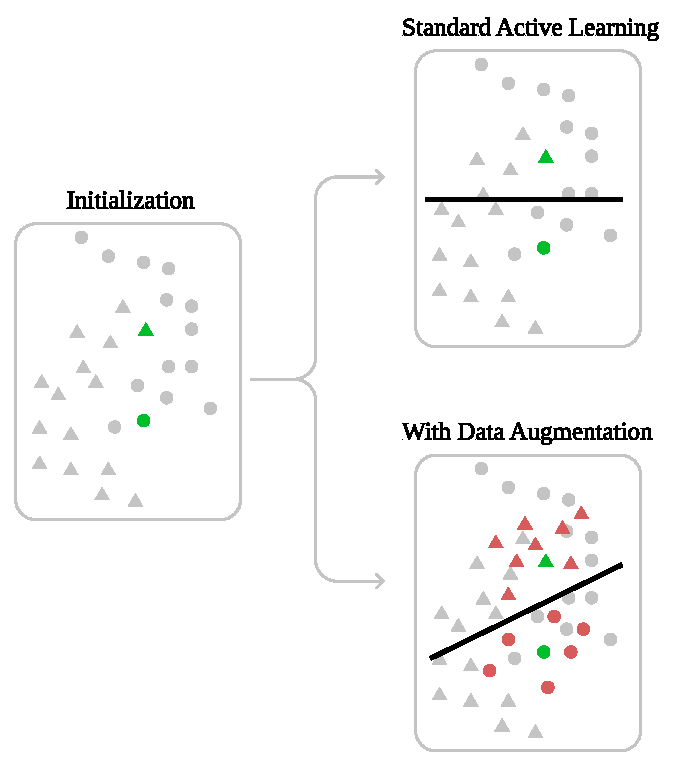
\includegraphics{../analysis/graphical_abstract}
\end{graphicalabstract}

%%Research highlights
\begin{highlights}
    \item We propose a new Active Learning framework that leverages
        hyperparameter optimization and data augmentation techniques;
    \item The use of data augmentation in Active Learning is sufficient to
        substancially improve the performance of an Active Learner, regardless of the
        choice of dataset/domain, classifier or metric.
    \item In most scenarios, the proposed method outperformed classifiers
        trained in fully supervised settings while using less data.
\end{highlights}

\begin{keyword}
Active Learning \sep\@ Data Augmentation \sep\@ Oversampling
\end{keyword}

\end{frontmatter}

\linenumbers%

\section{Introduction}~\label{sec:introduction}


The importance of training robust ML models with minimal data requirements is
substantially increasing~\cite{Nath2021, Sverchkov2017, Li2012}. Although the
growing amount of valuable data sources and formats being developed and
explored is affecting various domains~\cite{Li2021}, this data is often
unlabeled. Only a small amount of the data being produced and stored can be
useful \hl{for} supervised learning tasks. Additionally, it's important to note that
labeling data for specific Machine Learning (ML) projects is often difficult
and expensive, especially when data-intensive ML techniques are involved
(\textit{e.g.,} Deep Learning classifiers)~\cite{Nath2021}. In this scenario,
labeling the full dataset becomes impractical, time-consuming\hl{,} and expensive.
\hl{T}wo different ML techniques\hl{ a}ttempt to address this problem:
Semi-Supervised Learning (SSL) and Active Learning (AL). Even though they
address the same problem, the two follow different approaches. SSL focuses on
observations with the most certain predictions, whereas AL focuses on
observations with the least certain predictions~\cite{Simeoni2020}.

SSL attempts to use a small, predefined set of labeled and unlabeled data to
produce a classifier with superior performance. This method uses the unlabeled
observations to help define the classifier's decision
boundaries~\cite{Van2020}. Simultaneously, the amount of labeled data required
to reach a given performance threshold is also reduced. It is a special case
of ML because it falls between the supervised and unsupervised learning
perspectives. \hl{AL}, instead of optimiz\hl{ing} the informativeness of
a\hl{n existing} training set, \hl{it expands} the dataset \hl{to include} the
most informative and/or representative observations~\cite{Sener2018}. It
\hl{is} an iterative process where \hl{a} supervised model \hl{is trained}
\hl{and simultaneously} identifies \hl{the most informative} unlabeled
observations\hl{ to} increase the performance of that classifier. The
combination of SSL with AL has been explored in the past, achieving
state-of-the-art results~\cite{Leng2013}.
 
Several studies have pointed out the limitations of AL within an Imbalanced
Learning context~\cite{Yu2019}. With imbalanced data, AL approaches frequently
have low performance, high \hl{computational} time, or\hl{ }data annotation
costs.  Studies addressing this issue tend to adopt classifier-level
modifications, such as the Weighted Extreme Learning Machine~\cite{Yu2019,
Zong2013, Qin2021}. However, classifier or query function-level modifications
(See Section~\ref{sec:active_learning_methods}) have limited applicability
since a universally good AL strategy has not been found~\cite{Sener2018}.
Other methods address imbalance learning by weighing the observations as a
function of the observation's class imbalance ratio~\cite{Liu2021}.
Alternatively, other methods\hl{ }reduce the imbalanced learning bias
by combining Informative and Representative-based query approaches (see
Section~\ref{sec:active_learning_methods})~\cite{Tharwat2020}. Another
approach to deal with imbalanced data and data scarcity, in general, is data
augmentation. This approach has the advantage of being\hl{
}classifier-agnostic\hl{, }potentially reduces the imbalanced learning
bias\hl{, and also} work\hl{s} as a regularization method in data-scarce
environments, such as AL implementations~\cite{Kim2021}. However, most recent
studies\hl{ }improve the AL performance \hl{by modifying the design/choice of}
the classifier and query functions used.
 
The usage of data augmentation in AL is not new. The literature found on the
topic (see Section~\ref{sec:data_augmentation_in_al}) focuses on either image
classification or Natural Language Processing and uses Deep Learning-based
data augmentation to improve the performance of neural network architectures
in AL\@. These methods, although showing promising results, represent a
limited perspective of the potential of data augmentation in a real\hl{-}world
setting. First, \hl{using} Deep Learning in an iterative setting requires\hl{
}access \hl{to} significant computational power. Second, the\hl{se models tend
to use sophisticated} data augmentation
methods\hl{,} whose implementation may not be
accessible to the non-sophisticated user. Third, the studies found on the
topic are specific to the domain, classifier and data augmentation method.
Consequently, the direct effect of data augmentation is unclear: these studies
implement different neural network-based techniques for different
classification problems, whose performance may be attributed to various
elements within the AL framework.

In this study, we explore the effect of data augmentation in AL in a
context-agnostic setting, along with two different data augmentation policies:
\hl{oversampling} (where the amount of data generated for each class equals
the amount of data belonging to the majority class) and non-constant data
augmentation policies (where the amount of data generated exceeds the amount
of data belonging to the majority class in varying quantities) between
iterations. We start by conceptualizing the AL framework and each of its
elements, as well as the modifications involved to implement data augmentation
in the AL iterative process. We argue that simple, non-domain specific data
augmentation heuristics are sufficient to improve the performance of AL
implementations, without the need to resort to deep learning-based data
augmentation algorithms.

When compared to the standard AL framework, the proposed framework contains
two additional components: the Generator and the Hyperparameter Optimizer. We
implement \hl{a modified version of }Geometric Synthetic Minority Oversampling
Technique (G-SMOTE)~\cite{Douzas2019} as a data augmentation method with an
optimized generation policy (explained in
Section~\ref{sec:data_augmentation}). The hyperparameter optimization module
is used to find the best data \hl{augmentation} policy at each iteration. We test the
effectiveness of the proposed method in 10 datasets of different domains. We
implement 3 AL frameworks (standard, \hl{oversampling} and varying
data augmentation) using 4 different classifiers, 3 different performance
metrics and calculate 2 AL-specific performance metrics. 

The rest of this manuscript is structured as follows:
Section~\ref{sec:active_learning_methods} describes the state-of-the-art in
AL\@. Section~\ref{sec:data_augmentation} describes the state-of-the-art in Data
Augmentation. Section~\ref{sec:proposed_method} describes the proposed method.
Section~\ref{sec:methodology} describes the methodology of the study's
experiment. Section~\ref{sec:results_discussion} presents the results obtained
from the experiment, as well as a discussion of these results.
Section~\ref{sec:conclusion} presents the conclusions drawn from this study.
 
\section{Background}

\subsection{Active Learning}~\label{sec:active_learning_methods}

\hl{This paper focuses on pool-based AL methods as defined
in}~\cite{katz2021improved}. \hl{The goal of AL models is to maximize the
performance of a classifier, $f_{c}$,  while annotating as least
observations, $x_i$, as possible. They use a data pool, $\mathcal{D}$, where
$\mathcal{D} = \mathcal{D}_{lab} \cup \mathcal{D}_{pool}$ and
$|\mathcal{D}_{pool}| \gg |\mathcal{D}_{lab}|$.  $\mathcal{D}_{pool}$ and
$\mathcal{D}_{lab}$ refer to the sets of unlabeled and labeled data,
respectively.  Having a budget of $T$ iterations (where $t = 1, 2, \ldots, T$)
and $n$ annotations per iteration, at iteration $t$, $f_c$ is trained using
$\mathcal{D}_{lab}^t$ to produce, for each $x_i \in \mathcal{D}_{pool}^t$, an
uncertainty score using an acquisition function $f_{acq}(x_i;f_c)$. These
uncertainty scores are used to annotate the $n$
observations with highest ucertainty from $\mathcal{D}_{pool}^t$ to form
$\mathcal{D}_{new}^t$. The iteration ends with the update of
$\mathcal{D}_{lab}^{t+1} = \mathcal{D}_{lab}^t \cup \mathcal{D}_{new}^t$ and
$\mathcal{D}_{pool}^{t+1} = \mathcal{D}_{pool}^t \setminus
\mathcal{D}_{new}^t$}~\cite{Su2020, Sverchkov2017}. \hl{This
process is shown in Figure}~\ref{fig:al_iteration}.

\hl{Before the start of the iterative process, assuming 
$\mathcal{D}_{lab}^{t=0} = \emptyset$, the data used to populate
$\mathcal{D}_{lab}^{t=1}$ is typically collected randomly from
$\mathcal{D} = \mathcal{D}_{pool}^{t=0}$ and is labeled by a
supervisor}~\cite{Fonseca2021, Yoo2019, Aghdam2019}\hl{.} 

\begin{figure}[H]
	\centering
	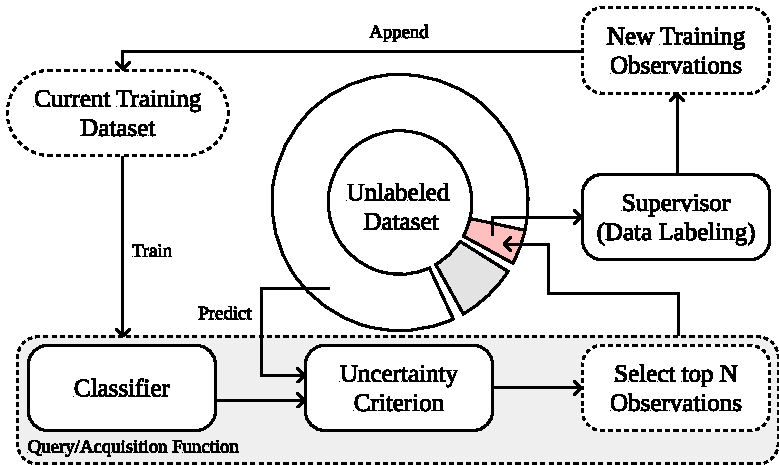
\includegraphics[width=.75\linewidth]{../analysis/al_iteration}
    \caption{%
        Diagram depicting a typical AL iteration. In the first iteration, the
        training set collected during the initialization process becomes the
        ``Current Training Dataset''.
    }~\label{fig:al_iteration}
\end{figure}

\hl{Research focused on AL} has typically been focused on the
specification of \hl{$f_{acq}$ and} domain-specific
applications. \hl{Acquisition} functions can be divided into two different
categories~\cite{Gu2021, Kumar2020}: 

\begin{enumerate}

    \item Informative-based query strategies. These strategies use the
        classifier's output to assess the importance of each observation
        towards the performance of the classifier. These strategies focus on
        quantifying the class uncertainty of the unlabeled observations.
        Since these techniques do not account for the relationships between
        the unlabeled observations and treats each observation
        independently~\cite{Fu2013}.

    \item Representative-based query strategies. These strategies estimate the
        optimal set of observations that will optimize the classifier's
        performance. This strategy contains 3 main approaches: Density-based,
        Diversity-based and Exploration of graph structures. Although this
        method addresses the problem of sampling bias and redundant instance
        selection, these strategies typically require more observations in
        order to reach the desired classification
        performance~\cite{Kumar2020}.

\end{enumerate}

Although there are significant contributions towards the development of more
robust query functions and classifiers in AL, modifications to AL's basic
structure is rarely explored. In~\cite{Yoo2019} the authors introduce a loss
prediction module in the AL framework to replace the uncertainty criterion.
This model implements a second classifier to predict the expected loss of the
unlabeled observations (using the actual losses collected during the training
of the original classifier) and return the unlabeled observations with the
highest expected loss. \hl{However}, this contribution is specific to neural
networks (and more specifically, to deep neural networks)\hl{and was only tested
for image classification}.

\pagebreak

In~\cite{Simeoni2020} the authors propose the usage of semi-supervised
learning during both the initialization of the AL and the iterative process as
well. However, this method was proposed specifically for deep learning
applications. In~\cite{Fonseca2021}, the authors introduce the generator
element in the AL framework (discussed in Section~\ref{sec:proposed_method})
using an oversampling method, showing that this method effectively addresses
the limitations of imbalanced learning. However, this method was implemented
specifically in the Remote Sensing domain and used an oversampling strategy
without consideration for the actual amount of artificial data generated,
which may limit its performance.
 
\subsection{Query Strategies}

A query strategy/function encompasses all the steps prior to the data labeling
within an AL iteration. They focus on finding the observations'
informativeness, representativeness or both~\cite{Gu2021, Kumar2020}.
Representative query strategies are generally less efficient in data selection
than Informative query strategies~\cite{Kumar2020}. However, recent research
often use representative approaches alongside informative
approaches~\cite{Gu2021, Samat2016}. Representative query strategies are
explored via 3 main approaches~\cite{Kumar2020}: 

\begin{enumerate}
    \item Density-based, which select representative observations from high
        density regions.~\cite{Huang2014, Li2012, Ienco2013} used a
        density-based approach using clustering algorithms to select the
        observations closest to the centroid of each cluster. 
    \item Diversity-based, which select the N observations at each iteration
        that maximize the diversity in the training data. The diversity-based
        approach was developed to avoid the selection of redundant
        observations in batch-mode learning~\cite{Brinker2003}.
    \item Graph-based, which find the most representative nodes and edges of a
        graph network~\cite{Jia2019}. Since these methods are specific to
        graph network data, they have a more limited applicability.
\end{enumerate}

Informative query strategies, unlike representative query strategies, do not
account for the structure of the unlabeled dataset. As a result, this type of
strategy may lead to the inefficient selection of observations (\textit{i.e.,}
redundant observations with similar profiles)~\cite{Kumar2020}. Research on
more robust selection criteria attempts to address the efficiency problem.
This is motivated by the importance of the selection criteria in AL's
iterative process~\cite{Rosario2020}. Specifically, Settles~\cite{Settles2011}
observed that in some datasets informative query strategies fail to outperform
the random selection of observations. Generally, the Random Selection query
method is used as a baseline. This method disregards the class membership
probabilities produced by the classifier and returns N random points from the
dataset without following any specific criteria.

A frequently used query strategy is Uncertainty Sampling, originally proposed
in~\cite{Lewis1994}. Using this method, the estimation of an observation's
uncertainty is based on the target class with the highest probability ($p_a$,
according to the classifier) and the uncertainty is calculated as $1-p_a$.
However, since this method dismissed the classifier's predictions on the
remaining labels, the Breaking Ties criterion was proposed to address this
limitation for multiclass problems~\cite{Luo2005}. This method uses the two
target classes with highest probability ($p_a$ and $p_b$, according to the
classifier) and the uncertainty is calculated as $p_a - p_b$ (in this case,
the lower the output value, the higher the uncertainty). Recent variants of
the Breaking Ties criterion, such as the Modified Breaking Ties, attempted to
fix some limitations of the original method~\cite{Liu2018, Li2012a}.

Another common informative query strategy is the calculation of Shannon's
Entropy. This metric measures the level of uncertainty
based on the probabilities of a set of possible events. Its formula is given
by $H(p)=-\sum_{i=0}^n{p_i\log_2{p_i}}$, having $p$ as the set of
probabilities of all target classes. The application of the Entropy
uncertainty criterion is also frequently applied in Deep Active
Learning~\cite{Aghdam2019}. Other Entropy-based methods were also developed
for more specific applications. For example, an ensemble querying approach
known as Entropy Querying-by-Bagging uses the predictions of all estimators to
find the maximum entropy of each observation~\cite{Abe1998}.

The Query by Committee (QBC) strategy was developed to address ensemble
classifiers. It is a disagreement based strategy attempts to maximize the
information gain at each iteration by computing the disagreement of the
predictions over the estimators that form the ensemble. The Entropy
Querying-by-Bagging and Query-by-Boosting methods are also ensemble
strategies. Query by boosting and bagging methods were found to achieve a good
performance over various datasets~\cite{Melville2004}, while the performance
between the two strategies appears to differ significantly across various
scenarios~\cite{Bloodgood2018}.

Other classifier-specific query strategies were also developed for different
applications. However, these methods have the disadvantage of depending on the
classifier being used. For example, Margin Sampling is a well studied strategy
that uses a Support Vector Machine as its classifier in order to select the
unlabeled observations closest to its decision boundaries~\cite{Kumar2020}.
Although, since this method is known to lead to the excessive selection of
observations in dense regions~\cite{Zhou2014}, it was improved in various
ways. In~\cite{Zhou2014} the authors extend this strategy by applying the
manifold-preserving graph reduction algorithm beyond the normal Margin
Sampling method.
 
\section{Data Augmentation Methods}~\label{sec:data_augmentation}

Data Augmentation methods expand the training dataset by introducing new and
informative observations~\cite{Behpour2019}. The production of artificial data
may be done via the introduction of perturbations on the
input~\cite{Zhong2020}, feature~\cite{DeVries2017} or output
space~\cite{Behpour2019}. Data Augmentation methods may be divided into
Heuristic and Neural Network-based approaches~\cite{Shorten2019}. In addition,
they may also be distinguished based on its data generation policy, whether
local (considers a local/specific subset of the dataset) or global (considers
the overall distribution of the training dataset).
Figure~\ref{fig:data_augmentation_taxonomy} shows the general taxonomy of
Heuristic Data Augmentation methods. Finding the appropriate Data Augmentation
method generally depends on the domain~\cite{DeVries2017}, although some
studies discuss which methods are more appropriate according to the
domain~\cite{Shorten2019, Iwana2021, Wong2016}.

\begin{figure}[H]
	\centering
	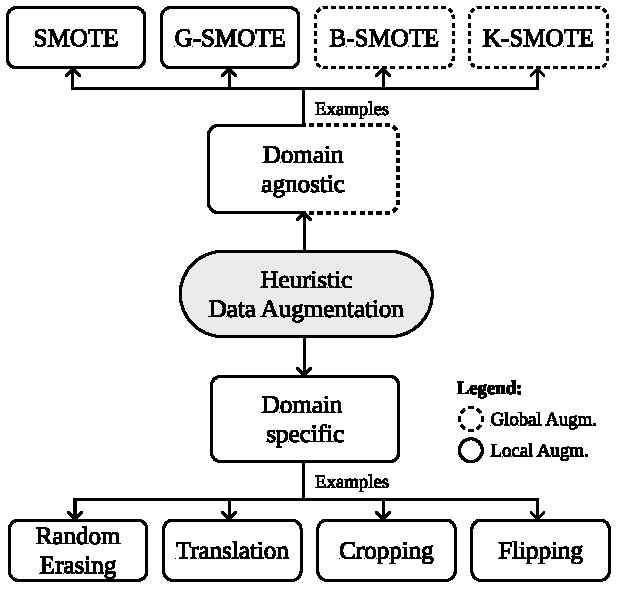
\includegraphics[width=.55\linewidth]{../analysis/data_augmentation_taxonomy}
    \caption{%
        Schema containing a general Heuristic Data Augmentation taxonomy.
    }~\label{fig:data_augmentation_taxonomy}
\end{figure}

Heuristic approaches attempt to generate new and relevant observations through
the application a predefined procedure, usually incorporating some degree of
randomness~\cite{Kashefi2020}. Since these methods typically occur in the
input space, they require less data and computational power when compared to
Neural Network methods. Neural Network approaches, on the other hand, map the
original input space into a lower-dimensional representation, known as the
feature space~\cite{DeVries2017}. The generation of artificial data occurs in
the feature space and is reconstructed into the input space. Although these
methods allow the generation of less noisy data in high-dimensional contexts
and more plausible artificial data, they are significantly more
computationally intensive. Considering the scope of this paper (the paper's
contribution is described in Sections~\ref{sec:introduction}
and~\ref{sec:proposed_method}), the computational power available for this
experiment and the breadth of datasets used in our experimental procedure, we
will focus on domain-agnostic heuristic data augmentation methods.

While some techniques may depend on the domain, others are domain-agnostic.
For example, Random Erasing~\cite{Zhong2020}, Translation, Cropping and
Flipping are image data-specific augmentation methods. Other methods, such as
most of the variants of the Synthetic Minority Oversampling TEchnique
(SMOTE)~\cite{Chawla2002}, may be considered domain agnostic. However, SMOTE
methods were originally developed as oversamplers, whose goal is to balance
the class frequencies of the target variable in the training dataset and
address the class imbalance bias~\cite{Fonseca2021ksmote}. Therefore,
oversampling methods may be considered a subset of Data Augmentation. Data
Augmentation strategies may follow varying augmentation strategies, which does
not necessarily depend on the target class distribution. An example of the
differences among general data augmentation and oversampling generation
strategies is shown in Figure~\ref{fig:augmentation_strategies}.

\begin{figure}[H]
	\centering
	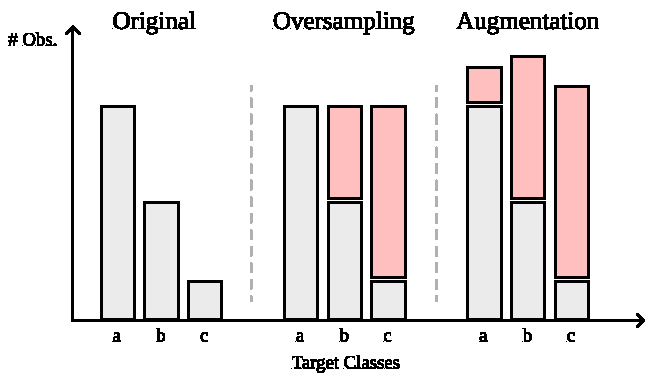
\includegraphics[width=.6\linewidth]{../analysis/augmentation_strategies}
    \caption{%
        Examples of data augmentation Strategies. The salmon-colored bars
        represent artificial data using the normal oversampling (center group) and
        an example of augmentation (right group) strategies.
    }~\label{fig:augmentation_strategies}
\end{figure}

The simplest approach found in the literature is randomly duplicating existing
training observations. As a non-informed data generation method, although
simple to implement, it increases the risk of overfitting and generally
performs worse than other informed heuristic
methods~\cite{Douzas2019imbalanced}.

The SMOTE method generates artificial data via the linear interpolation
between a random observation and one of its $k$-nearest neighbors (also
randomly selected)~\cite{Chawla2002}. Although simple and effective, it also
contains several limitations which motivated the development other variants,
discussed below. Specifically, its selection mechanism does not consider the
global structure of the dataset while its generation mechanism introduces
little variability into the training dataset~\cite{Douzas2019}.
Borderline-SMOTE (B-SMOTE)~\cite{Han2005} improves the selection mechanism by
attributing a larger importance to the observations closer to the decision
boundaries. The selected observations are used to run the SMOTE method in
order to produce better defined decision boundaries. A more recent improvement
of the selection mechanism is K-means SMOTE (K-SMOTE)~\cite{Douzas2018}. This
method uses a clustering-based approach to overcome imbalances between and
within classes, while considering the densities of each region of the input
space.

\begin{figure}[H]
	\centering
	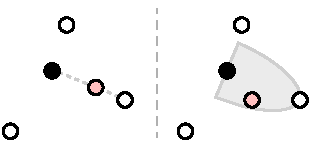
\includegraphics[width=.45\linewidth]{../analysis/smote_vs_gsmote}
    \caption{%
        Examples of data generation using SMOTE and G-SMOTE\@. In this
        example, both G-SMOTE's deformation and truncation parameters assume
        values around $0.5$.
    }~\label{fig:smote_vs_gsmote}
\end{figure}

G-SMOTE~\cite{Douzas2019} modifies SMOTE's generation mechanism. Instead of
generating an observation as a linear combination between 2 others, it
generates observations within an hypersphere defined using the selected
observation as its center and one of its nearest neighbors as its boundary.
The hypersphere contains two hyperparameters, the truncation and deformation
factors, which limit the area of the hypersphere. The difference between SMOTE
and G-SMOTE is shown in Figure~\ref{fig:smote_vs_gsmote}.
Reference~\cite{Douzas2019imbalanced} found that G-SMOTE outperforms various
state-of-the-art oversamplers.
 
\subsection{Data Augmentation in Active Learning
}~\label{sec:data_augmentation_in_al}

As found in Section~\ref{sec:active_learning_methods}, the improvement of the
AL framework found in the literature are mostly focused on modifications of
the classifier or query strategy. However, a few recent AL applications
implementing data augmentation were found. The method proposed
in~\cite{Kim2021}, Look-Ahead Data Acquisition for Deep Active Learning,
implement image data specific data augmentation to train a deep learning
classifier. However, in this study, data augmentation is based on the
unlabeled observations and occurs before the unlabeled data selection.
In~\cite{Ma2020} the proposed AL method was designed specifically for image
data classification, where a deep learning model was implemented as a
classifier, but its architecture is not described. Other AL frameworks
implementing data augmentation may also be found for Natural Language
Processing applications~\cite{Quteineh2020, Li2021framework}. However, these
methods were designed for specific within that domain and are not necessarily
transferrable to other domains or tasks.
 
\section{Proposed Method}~\label{sec:proposed_method}

Based on the literature found on AL, most of the contributions and novel
implementations of AL algorithms focused on the improvement of the
choice/architecture of the classifier or the improvement of the uncertainty
criterion. In addition, the resulting classification performance of AL-trained
classifiers is frequently inconsistent and marginally improve the
classification performance when compared to classifiers trained over the full
training set. Finally, in~\cite{Fonseca2021} the authors also found a
significant variability of the data selection efficiency during different runs
of the AL iterative process. In that study the authors proposed a new element
within the AL framework, the generator, which was able to marginally reduce
the variability previously identified. However, this modification was applied
in a Land Use/Land Cover context which contains specific characteristics that
are not necessarily found in other supervised learning problems. Specifically,
\hl{these types of datasets are high dimensional and have limited data
variability within each class} (\textit{i.e.,} cohesive spectral signatures
within classes) due to their geographical proximity. Furthermore, the
implementation of the generator was done using a simple oversampling
augmentation policy, which limits the possibility of employing other
techniques with an undefined target amount of data generated at each
iteration.
 
This paper provides a context-agnostic AL framework towards the integration of
Data Augmentation within AL, with the following contributions:

\begin{enumerate}
    \item Improvement of the AL framework by introducing a parameter
        tuning stage using only the labeled dataset available at the current
        iteration (\textit{i.e.,} no labeled hold-out set is needed).
    \item Generalization of the generator module proposed
        in~\cite{Fonseca2021} from oversampling techniques to any other data
        augmentation mechanism and/or policy.
    \item Implementation of data augmentation outside of the Deep AL realm,
        which was not previously found in the literature.
    \item Analysis of the impact of Data Augmentation and Oversampling
        in AL over 10 different datasets of different domains, while
        comparing them with the standard AL framework.
\end{enumerate}

The proposed iterative process of the AL framework is depicted in
Figure~\ref{fig:al_proposed}. The generator element becomes an additional
source of data and is expected to introduce additional data variability into
the training dataset. This should allow the classifier to generalize better
and perform more consistently over unseen observations. However, in this
scenario, the amount of data to generate per class at each iteration is
unknown. Consequently, the hyperparameter tuning step was introduced to
estimate the optimal data augmentation policy at each iteration. In our
implementation, this step uses the current training dataset to perform an
exhaustive search over specified parameters of the generator, tested over a
5-fold cross validation method. The best augmentation policy found is used
to train the iteration's classifier in the following step.

\begin{figure}[H]
	\centering
	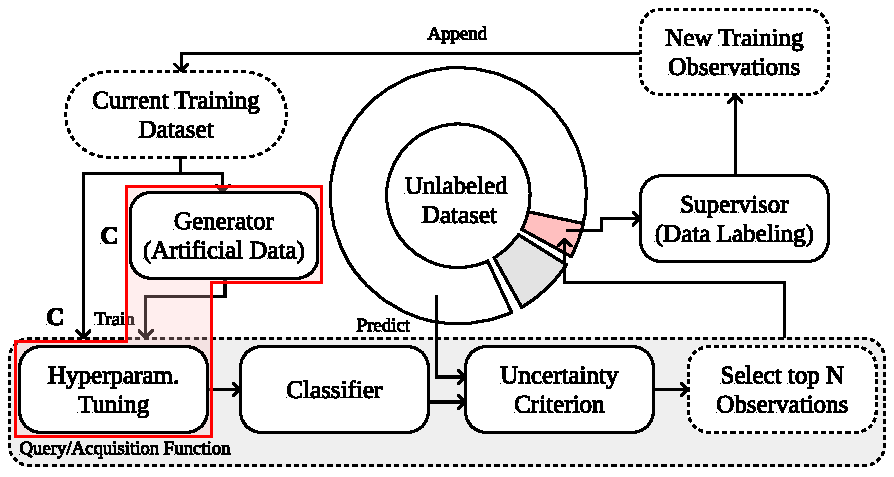
\includegraphics[width=.75\linewidth]{../analysis/al_proposed}
    \caption{%
        Diagram depicting the proposed AL iteration. The proposed
        modifications are marked with a boldface ``C''.
    }~\label{fig:al_proposed}
\end{figure}

To show the effectiveness of data augmentation in an AL implementation, we
implemented a simple modification of the G-SMOTE algorithm. This modification
facilitates the usage of G-SMOTE beyond its original oversampling purposes. In
this paper, the data augmentation strategies used ensure the all the class
frequencies are balanced. Furthermore, the amount of artificial data produced
for each class is defined by the \textit{augmentation factor}, which
represents a percentage of the majority class $C_{maj}$ (\textit{e.g.,} an
augmentation factor of $1.2$ will ensure there are $count(C_{maj}) \times 1.2$
observations in every class). In this paper's experiment, the data generation
mechanism is similar to the one in~\cite{Fonseca2021}. This allows the direct
comparison of the two frameworks and establish a causality of the performance
variations to the data generation mechanism (\textit{i.e.,} augmentation vs
normal oversampling) and hyperparameter tuning steps.

\begin{figure}[H]
	\centering
	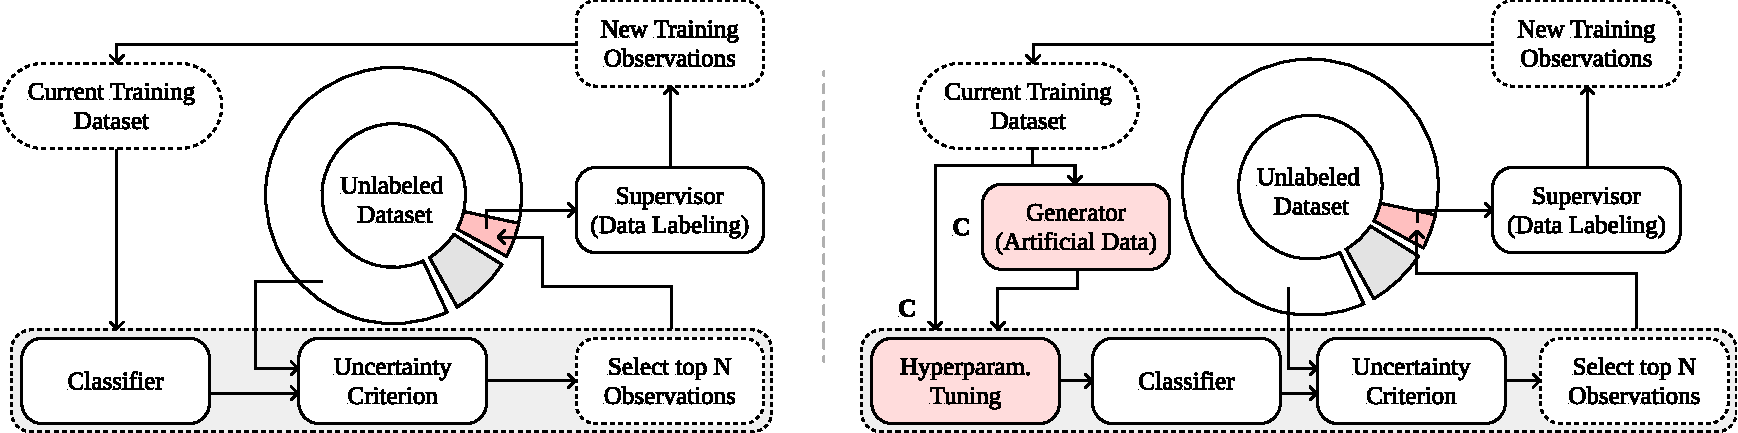
\includegraphics[width=\linewidth]{../analysis/al_comparison}
    \caption{%
        Simplified diagrams highlighting the differences between the proposed
        and standard AL iterations. The proposed modifications are highlight
        in red and marked with a boldface ``C''.
    }~\label{fig:al_comparison}
\end{figure}

The comparison of diagrams between the proposed and standard AL frameworks is
shown in Figure~\ref{fig:al_comparison}. In the proposed framework, we (1)
generalize the generator module to accept any data augmentation method or
policy and (2) a hyperparameter tuning module to estimate the optimal data
augmentation policy. This framework was designed to be task-agnostic.
Specifically, any data augmentation method (domain specific or not) may be
used, as well as any other parameter search method. It is also expected to be
compatible with other AL modifications, including the ones that do not affect
solely the classifier or uncertainty criterion, such as the one proposed
in~\cite{Yoo2019}.
 
\section{Methodology}~\label{sec:methodology}

This section describes the different elements included in the experimental
procedure. The datasets used were acquired in open data repositories and its
sources and preprocessing steps are defined in Subsection~\ref{sec:datasets}.
The choice of classifiers used in the experiment are defined in
Subsection~\ref{sec:machine_learning_algorithms}. The metrics chosen to
measure AL performance and overall classification performance are defined in
Subsection~\ref{sec:evaluation_metrics}. The experimental procedure is
described in Subsection~\ref{sec:experimental_procedure}. The implementation
of the experiment and resources used to do so are described in
Subsection~\ref{sec:software_implementation}.

The methodology developed serves 2 purposes: (1) Compare classification
performance once all the AL procedures are completed (\textit{i.e.,} optimal
performance of a classifier trained via iterative data selection) and (2)
Compare the amount of data required to reach specific performance thresholds
(\textit{i.e.,} number of AL iterations required to reach similar
classification performances).
 
\subsection{Datasets}~\label{sec:datasets}

The datasets used to test the proposed method are publicly available in open
data repositories. Specifically, they were retrieved from
\href{https://www.openml.org/}{OpenML} and the
\href{https://archive.ics.uci.edu/}{UCI Machine Learning Repository}. They
were chosen considering different domains of application, imbalance ratios,
dimensionality and number of target classes, all of them focused on
classification tasks. The goal is to demonstrate the performance of the
different AL frameworks in various scenarios and domains. The data
preprocessing approach was similar across all datasets.
Table~\ref{tab:datasets_description} describes the key properties of the 10
preprocessed datasets where the experimental procedure was applied. 
 
\begin{table}[H]
    \centering
    \addtolength{\leftskip} {-3cm}
    \addtolength{\rightskip}{-3cm}
    \pgfplotstabletypeset[
        col sep=comma,
        string type,
        every head row/.style={%
            before row=\toprule,
            after row=\midrule
        },
        every last row/.style={after row=\bottomrule},
    ]{../analysis/datasets_description.csv}
    \caption{\label{tab:datasets_description}
        Description of the datasets collected after data preprocessing. The
        sampling strategy is similar across datasets. Legend: (IR) Imbalance
        Ratio
    }
\end{table}

The data preprocessing pipeline is depicted as a flowchart in
Figure~\ref{fig:data_preprocessing}. The missing values are removed from each
dataset by removing the corresponding observations. This ensures that the
input data in the experiment is kept as close to its original form as
possible. The non-metric features (\textit{i.e.,} binary, categorical and
ordinal variables) were removed since the application of G-SMOTE is limited to
continuous and discrete features. The datasets containing over 2000
observations were downsampled in order to maintain the datasets to a
manageable size. The data sampling procedure preserves the relative class
frequency of the dataset, in order to maintain the Imbalance Ratio (IR)
originally found in each dataset (where $IR =
\frac{count(C_{maj})}{count(C_{\min})}$). The remaining features of each
dataset are scaled to the range of $[-1, 1]$ to ensure a common range across
features.

\begin{figure}[H]
	\centering
	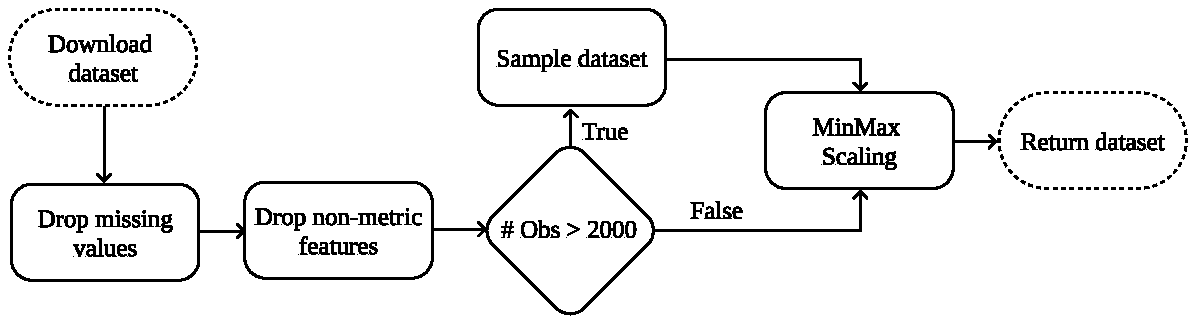
\includegraphics[width=1\linewidth]{../analysis/data_preprocessing}
    \caption{%
        Data preprocessing pipeline.
    }~\label{fig:data_preprocessing}
\end{figure}

The preprocessed datasets were stored into a SQLite database file and is
available along with the experiment's source code in the GitHub repository of
the project (see Subsection~\ref{sec:software_implementation}).
 
\subsection{Machine Learning Algorithms}~\label{sec:machine_learning_algorithms}

We used a total of 4 classification algorithms and a heuristic data
augmentation mechanism. The choice of classifiers was based on the popularity
and family of the classifiers (tree-based, nearest neighbors-based,
ensemble-based and linear models). Our proposed method was tested using a
Decision Tree (DT)~\cite{Wu1975}, a K-nearest neighbors classifier
(KNN)~\cite{Cover1967}, a Random Forest Classifier (RF)~\cite{Ho1995} and a
Logistic Regression (LR)~\cite{Nelder1972}. Since the target variables are
multi-class, the LR classifier was implemented using the one-versus-all
approach. The predicted class is assigned to the label with the highest
likelihood.
 
The oversampler G-SMOTE was used as a data augmentation method. The typical
data generation policy of oversampling methods is to generate artificial
observations on non-majority classes such that the number of majority class
observations matches those of each non-majority class. We modified this data
generation policy to generate observations for all classes, as a percentage of
the number of observations in the majority class. In addition, the original
G-SMOTE algorithm was modified to accept data selection probabilities based on
classification uncertainty. These modifications are discussed in
Section~\ref{sec:proposed_method}.

Every AL procedure was tested with different selection criteria: Random
Selection, Entropy and Breaking Ties. The baseline used is the standard AL
procedure. As a benchmark, we add the AL procedure using G-SMOTE as a normal
oversampling method, as proposed in~\cite{Fonseca2021}. Our proposed method
was implemented using G-SMOTE as a data augmentation method to generate
artificial observations for all classes, while still balancing the class
distribution, as described in Section~\ref{sec:proposed_method}. 
 
\subsection{Evaluation Metrics}~\label{sec:evaluation_metrics}

Considering the imbalanced nature of the datasets used in the experiment,
commonly used performance metrics such as Overall Accuracy (OA), although
being intuitive to interpret, are insufficient quantify a model's
classification performance~\cite{Jeni2013}. The Cohen's Kappa performance
metric, similar to OA, is also biased towards high frequency classes since its
definition is closely related to the OA metric, making its behavior consistent
with OA~\cite{Fatourechi2008}. However, these metrics remain popular choices
for the evaluation of classification performance. Other performance metrics
like $Precision = \frac{TP}{TP+TN}$, $Recall = \frac{TP}{TP+FN}$ or
$Specificity = \frac{TN}{TN + FP}$ are calculated as a function of True/False
Positives (TP and FP) and True/False Negatives (TN and FN) and can be used at
a per-class basis instead. In a multiple dataset \hl{scenario} with varying
amount of target classes and meanings, comparing the performance of different
models using these metrics becomes impractical.
 
Based on the recommendations found in~\cite{Jeni2013, Kubat1997}, we used 2
metrics found to be less sensitive to the class imbalance bias, along with OA
as a reference for easier interpretability:

\begin{itemize}
    \item The Geometric-mean scorer (G-mean) consists of the geometric mean of
        Specificity and Recall~\cite{Kubat1997}. Both metrics are calculated
        in a multiclass context considering a one-versus-all approach. For
        multiclass problems, the G-mean scorer is calculated as its average
        per class values: 
        
        \begin{equation*}
            \textit{G-mean} = \sqrt{\overline{Sensitivity} \times
            \overline{Specificity}}
        \end{equation*}

    \item The F-score metric consists of the harmonic mean of Precision and
        Recall. The two metrics are also calculated considering a
        one-versus-all approach. The F-score for the multi-class case
        can be calculated using its average per class values~\cite{Jeni2013}:

        \begin{equation*}
            \textit{F-score}=2\times\frac{\overline{Precision} \times
            \overline{Recall}}{\overline{Precision} + \overline{Recall}}
        \end{equation*}

    \item The OA consists of the number of TP divided by the total amount of
        observations. Considering $c$ as the label for the different classes
        present in a target class, OA is given by the following formula:

        \begin{equation*}
            \textit{OA} = \frac{\sum\limits_{c}{\text{TP}_{c}}}{%
		    	      \sum\limits_{c}{(\text{TP}_{c}+\text{FP}_{c})}}
        \end{equation*}
\end{itemize}

The comparison of the performance of AL frameworks is based on its data
selection and augmentation efficacy. Specifically, an efficient data
selection/generation policy allows the production of classifiers with high
performance on unseen data while using as least non-artificial training data
as possible. To measure the performance of the different AL setups, we follow
the recommendations found in~\cite{Kottke2017}. The performance of an AL setup
will be compared using two AL-specific performance metrics:

\begin{itemize}

    \item Area Under the Learning Curve (AULC). It is the sum of the
        classification performance over a validation/test set of the
        classifiers trained of all AL iterations. To facilitate the
        interpretability of this metric, the resulting AULC scores are fixed
        within the range $[0, 1]$ by dividing the AULC scores by the total
        amount of iterations (\textit{i.e.}, the maximum performance area).

    \item Data Utilization Rate (DUR)~\cite{Reitmaier2013}. Measures the
        percentage of training data required to reach a given performance
        threshold, as a ratio of the percentage of training data required by
        the baseline framework. This metric is also presented as a percentage
        of the total amount of training data, without making it relative to
        the baseline framework. The DUR metric is measured at 45 different
        performance thresholds, ranging between $[0.10, 1.00]$ at a 0.02 step.

\end{itemize}
 
\subsection{Experimental Procedure}~\label{sec:experimental_procedure}

The evaluation of different active learners in a live setting is generally
expensive, time-consuming and prone to human error. Instead, a common practice
is to compare them in an offline environment using labeled
datasets~\cite{Kagy2019}. In this scenario, since the dataset is already
labeled, the annotation process is done at zero cost.
Figure~\ref{fig:experimental_procedure} depicts the experiment designed for
one dataset over a single run. 
 
A single run starts with the splitting of a preprocessed dataset in 5
different partitions, stratified according to the class frequencies of the
target variable using the K-fold Cross Validation method. During this run, an
active learner or classifier is trained 5 times using a different partition as
the Test set each time. For each training process, a Validation set containing
25\% of the subset is created and is used to measure the data selection
efficiency (\textit{i.e.,} AULC and DUR using the classification performance
metrics, specific to AL). Therefore, for a single training procedure, 20\% of
the original dataset is used as the Validation set, 20\% is used as the Test
set and 60\% is used as the Train set. The AL simulations and the classifiers'
training occur within the Train set. However, the classifiers used to find the
maximum performance classification scores are trained over the full Train set.
The AL simulations are run over a maximum of 50 iterations (including the
initialization step), adding 1.6\% of the training set each time
(\textit{i.e.,} all AL simulations use less than 80\% of the Train set). Once
the training phase is completed, the Test set classification scores are
calculated using the trained classifiers. For the case of AL, the classifier
with the optimal Validation set score is used to estimate the AL's optimal
classification performance over unseen data.

The process shown in Figure~\ref{fig:experimental_procedure} is repeated over
3 runs using different random seeds over the 10 different datasets collected.
The final scores of each AL configuration and classifier correspond to the
average of the 3 runs and 5-fold Cross Validation estimations (\textit{i.e.,}
the mean score of 15 fits, across 10 datasets).

\begin{figure}[H]
	\centering
	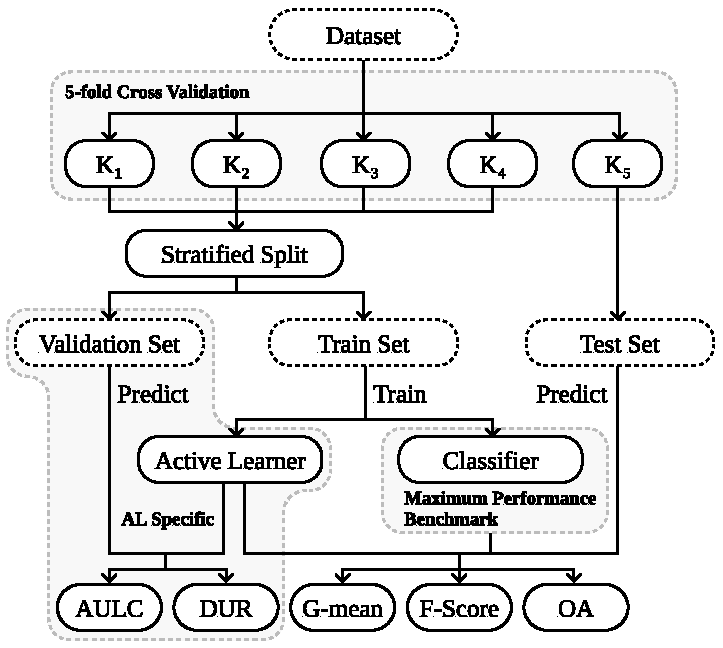
\includegraphics[width=.7\linewidth]{../analysis/experimental_procedure}
    \caption{%
        Experimental procedure flowchart. The preprocessed datasets are split
        into five folds. One of the folds is used to test the best found
        classifiers using AL and the classifiers trained using the entire
        training dataset (containing the remaining folds). The training set is
        used to run both the AL simulations as well as train the normal
        classifiers. The validation set is used to measure AL-specific
        performance metrics over each iteration. We use different subsets for
        overall classification performance and AL-specific performance to
        avoid data leakage.
    }~\label{fig:experimental_procedure}
\end{figure}

The hyperparameters defined for the AL frameworks, Classifiers and Generators
are shown in Table~\ref{tab:grid}. In the Generators table, we distinguish the
G-SMOTE algorithm working as a normal oversampling method from G-SMOTE-AUGM,
which performs generates additional artificial data on top of the usual
oversampling mechanism. Since the G-SMOTE-AUGM method is intended to be used
with varying parameter values (via within-iteration parameter tuning), the
parameters were defined as a list of various possible values.

\begin{table}[H]
	\centering
    \addtolength{\leftskip} {-3cm}
    \addtolength{\rightskip}{-3cm}
	\begin{tabular}{lll}
		\toprule
		Active Learners & Hyperparameters                   & Inputs                         \\
		\midrule
		Standard        & \# initial obs.\                  & 1.6\%                          \\
                        & \# additional obs.\ per iteration & 1.6\%                          \\
                        & max.\ iterations + initialization & 50                             \\
                        & evaluation metrics                & G-mean, F-score, OA            \\
                        & selection strategy                & Random, Entropy, Breaking Ties \\
                        & within-iteration param.\ tuning   & None                           \\
                        & generator                         & None                           \\
                        & classifier                        & DT, LR, KNN, RF                \\
        Oversampling    & generator                         & G-SMOTE                        \\
        Proposed        & generator                         & G-SMOTE-AUGM                   \\
                        & within-iteration param.\ tuning   & Grid Search K-fold CV          \\
		\toprule
		Classifier      &                                  &                                \\
		\midrule
        DT              & min.\ samples split              & 2                              \\
                        & criterion                        & gini                           \\
		LR              & maximum iterations               & 100                            \\
                        & multi class                      & One-vs-All                     \\
		                & solver                           & liblinear                      \\
                        & penalty                          & L2 (Ridge)                     \\
		KNN             & \# neighbors                     & 5                              \\
                        & weights                          & uniform                        \\
                        & metric                           & euclidean                      \\
		RF              & min.\ samples split              & 2                              \\
		                & \# estimators                    & 100                            \\
                        & criterion                        & gini                           \\
		\toprule
		Generator       &                                  &                                \\
		\midrule
		G-SMOTE         & \# neighbors                     & 4                              \\
                        & deformation factor               & 0.5                            \\
                        & truncation factor                & 0.5                            \\
		G-SMOTE-AUGM    & \# neighbors                     & 3, 4, 5                        \\
                        & deformation factor               & 0.5                            \\
                        & truncation factor                & 0.5                            \\
                        & augmentation factor              & $[1.1, 2.0]$ at 0.1 step       \\
		\bottomrule
	\end{tabular}
    \caption{\label{tab:grid}
        Hyperparameter definition for the active learners, classifiers and
        generators used in the experiment.
    }
\end{table}
 
\subsection{Software Implementation}~\label{sec:software_implementation}

The experiment was implemented using the Python programming language, along
with the Python libraries
\href{https://scikit-learn.org/stable/}{Scikit-Learn}~\cite{Pedregosa2011},
\href{https://imbalanced-learn.org/en/stable/}{Imbalanced-Learn}~\cite{JMLR:v18:16-365},
\href{https://geometric-smote.readthedocs.io/en/latest/?badge=latest}{Geometric-SMOTE}~\cite{Douzas2019},
\href{https://research-learn.readthedocs.io/en/latest/?badge=latest}{Research-Learn}
and
\href{https://mlresearch.readthedocs.io/en/latest/?badge=latest}{ML-Research}
libraries. All functions, algorithms, experiments and results are provided in
the \href{https://github.com/joaopfonseca/ml-research/}{GitHub repository of
the project}.

\section{Results \& Discussion}~\label{sec:results_discussion}

In a multiple dataset experiment, the analysis of results should not rely
uniquely on the average performance scores across datasets. The domain of
application and fluctuations of performance scores between datasets make the
analysis of these averaged results less accurate. Instead, it is generally
recommended the use of the mean ranking scores to extend the
analysis~\cite{Demsar2006}. Since mean performance scores are still intuitive
to interpret, we will present and discuss both results. The rank values are
assigned based on the mean scores of 3 different runs of 5-fold Cross
Validation (15 performance estimations per dataset) for each combination of
dataset, AL configuration, classifier and performance metric.
 
\subsection{Results}~\label{sec:results}

The average ranking of the AULC estimations of AL methods are shown in
Table~\ref{tab:aulc_ranks}. The proposed method almost always improves AL
performance and ensures higher data selection efficiency.
 
% % TODO: 
% % - Convert this table into a bar plot?
\begin{table}[H]
	\centering
    \addtolength{\leftskip} {-3cm}
    \addtolength{\rightskip}{-3cm}
    \pgfplotstabletypeset[
        col sep=comma,
        string type,
        every head row/.style={%
            before row=\toprule,
            after row=\midrule
        },
        every last row/.style={after row=\bottomrule},
    ]{../analysis/mean_std_aulc_ranks.csv}
    \caption{%
        Mean rankings of the AULC metric over the different datasets (10),
        folds (5) and runs (3) used in the experiment. The proposed method
        always improves the results of the original framework and on average
        almost always improves the results of the oversampling framework.
    }\label{tab:aulc_ranks}
\end{table}
 
Table~\ref{tab:aulc_scores} shows the average AULC scores, grouped by
classifier, Evaluation Metric and AL framework. The variation in performance
across active learners is consistent with the mean rankings found in
Table~\ref{tab:aulc_ranks}, while showing significant AULC score differences
between the proposed AL method and the oversampling AL method.

\begin{table}
	\centering
    \addtolength{\leftskip} {-3cm}
    \addtolength{\rightskip}{-3cm}
    \pgfplotstabletypeset[
        col sep=comma,
        string type,
        every head row/.style={%
            before row=\toprule,
            after row=\midrule
        },
        every last row/.style={after row=\bottomrule},
    ]{../analysis/mean_std_aulc_scores.csv}
    \caption{\label{tab:aulc_scores}
        Average AULC of each AL configuration tested. Each AULC score is
        calculated using the performance scores of each iteration in the
        validation set. By the end of the iterative process, each AL
        configuration used a maximum of 80\% instances of the 60\% instances
        that compose the training sets (\textit{i.e.,} 48\% of the entire
        preprocessed dataset).
    }
\end{table}

The average DUR scores were calculated for various G-mean thresholds, varying
between 0.1 and 1.0 at a 0.02 step (45 different thresholds in total).
Table~\ref{tab:optimal_data_utilization} shows the results obtained for these
scores starting from a G-mean score of 0.6 and was filtered to show only the
thresholds ending with 0 or 6. In most cases, the proposed method reduces the
amount of data annotation required to reach each G-mean score threshold.

\begin{table}
    \centering
    \addtolength{\leftskip} {-2cm}
    \addtolength{\rightskip}{-2cm}
    \pgfplotstabletypeset[
        col sep=comma,
        string type,
        every head row/.style={%
            before row=\toprule,
            after row=\midrule
        },
        every last row/.style={after row=\bottomrule},
    ]{../analysis/optimal_data_utilization.csv}
    \caption{\label{tab:optimal_data_utilization}
        Mean data utilization of AL algorithms, as a percentage of the
        training set.
    }
\end{table}

The DUR scores relative to the Standard AL method are shown in
Figure~\ref{fig:dur}. A DUR below 1 means that the Proposed/Oversampling
method requires less data than the Standard AL method to reach the same
performance threshold. For example, running an AL simulation using the KNN
classifier requires 69.6\% of the amount of data required by the Standard AL
method using the same classifier to reach an F-Score of 0.62 (\textit{i.e.,}
requires 30.4\% less data).

\begin{figure}
	\centering
	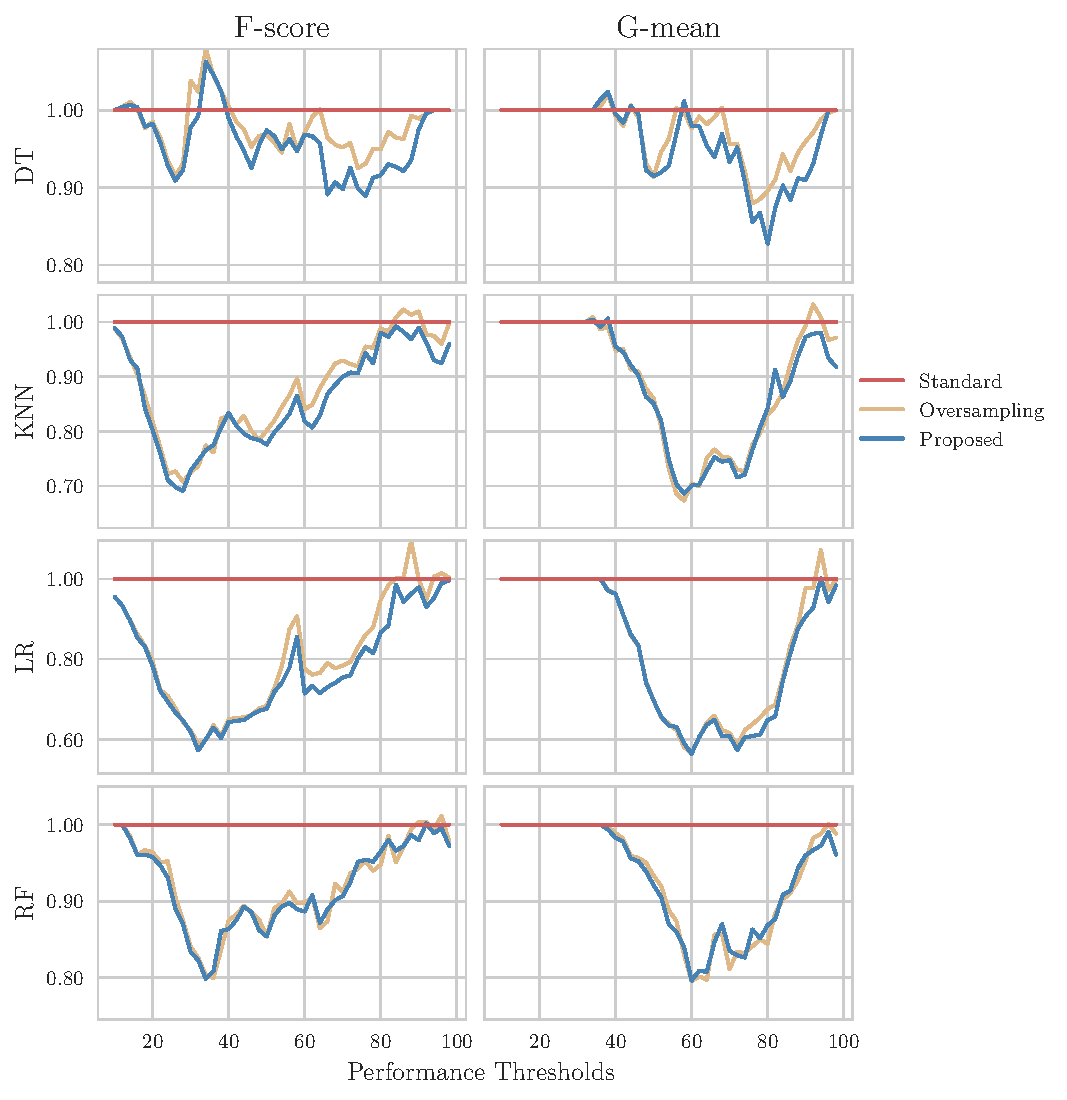
\includegraphics[width=1\linewidth]{../analysis/data_utilization_rate}
    \caption{%
        Mean data utilization rates. The y-axis shows the percentage of data
        (relative to the baseline AL framework) required to reach the
        different performance thresholds.
    }~\label{fig:dur}
\end{figure}

The mean optimal classification scores of AL methods and Classifiers (fully
labeled training set, without AL) is shown in
Table~\ref{tab:optimal_mean_std_scores}. The proposed AL method produces
classifiers that are almost always able to outperform classifiers using the
full training set (\textit{i.e.,} the ones labeled as MP).

\begin{table}
    \centering
    \addtolength{\leftskip} {-3cm}
    \addtolength{\rightskip}{-3cm}
    \pgfplotstabletypeset[
        col sep=comma,
        string type,
        every head row/.style={%
            before row=\toprule,
            after row=\midrule
        },
        every last row/.style={after row=\bottomrule},
    ]{../analysis/optimal_mean_std_scores.csv}
    \caption{\label{tab:optimal_mean_std_scores}
        Optimal classification scores. The Maximum Performance (MP)
        classification scores are calculated using classifiers trained using
        the entire training set.
    }
\end{table}

\subsection{Statistical Analysis}~\label{sec:statistical-analysis}

When checking for statistical significance in a multiple dataset context it is
important to account for the multiple comparison problem. Consequently, our
statistical analysis focuses on the recommendations found
in~\cite{Demsar2006}. Overall, we perform 3 statistical tests. The Friedman
test~\cite{Friedman1937} is used to understand whether there is a
statistically significant difference in performance between the 3 AL
frameworks. As post hoc analysis, the Wilcoxon signed-rank
test~\cite{Wilcoxon1945} was used to check for statistical significance
between the performance of the proposed AL method and the oversampling AL
method across datasets. As a second post hoc analysis, the
Holm-Bonferroni~\cite{Holm1979} method was used to check for statistical
significance between the methods using data generators and the Standard AL
framework across classifiers and evaluation metrics.
 
Table~\ref{tab:friedman_test} contains the \textit{p-values} obtained with the
Friedman test. The difference in performance across AL frameworks is
statistically significant at a level of $\alpha = 0.05$ regardless of the
classifier or evaluation metric being considered.

\begin{table}[H]
	\centering
    \pgfplotstabletypeset[
        col sep=comma,
        string type,
        every head row/.style={%
            before row=\toprule,
            after row=\midrule
        },
        every last row/.style={after row=\bottomrule},
    ]{../analysis/friedman_test.csv}
    \caption{%
        Results for Friedman test. Statistical significance is tested at a
        level of $\alpha = 0.05$. The null hypothesis is that there is no
        difference in the classification outcome across oversamplers.
    }\label{tab:friedman_test}
\end{table}

Table~\ref{tab:wilcoxon_test} contains the \textit{p-values} obtained with the
Wilcoxon signed-rank test. The proposed method was able to outperform both the
standard AL framework, as well as the AL framework using a normal oversampling
policy proposed in~\cite{Fonseca2021} with statistical significance in 9 out
of 10 datasets.

\begin{table}
	\centering
    \pgfplotstabletypeset[
        col sep=comma,
        string type,
        every head row/.style={%
            before row=\toprule,
            after row=\midrule
        },
        every last row/.style={after row=\bottomrule},
    ]{../analysis/wilcoxon_test.csv}
    \caption{%
        Adjusted p-values using the Wilcoxon signed-rank method. Bold values
        are statistically significant at a level of $\alpha = 0.05$. The null
        hypothesis is that the performance of the proposed framework is
        similar to that of the oversampling or standard framework.
    }\label{tab:wilcoxon_test}
\end{table}

The \textit{p-values} shown in Table~\ref{tab:holms_test} refer to the results
of the Holm-Bonferroni test. The proposed method's superior performance was
statistically significant for any combination of classifier and evaluation
metric. Simultaneously, the proposed method established statistical
significance in the 3 scenarios where the oversampling AL method failed to do
so.

\begin{table}
	\centering
    \pgfplotstabletypeset[
        col sep=comma,
        string type,
        every head row/.style={%
            before row=\toprule,
            after row=\midrule
        },
        every last row/.style={after row=\bottomrule},
    ]{../analysis/holms_test.csv}
    \caption{%
        Adjusted p-values using the Holm-Bonferroni method. Bold values are
        statistically significant at a level of $\alpha = 0.05$. The null
        hypothesis is that the Oversampling or Proposed method does not
        perform better than the control method (Standard AL framework).
    }\label{tab:holms_test}
\end{table}

\subsection{Discussion}~\label{sec:sub_discussion}

In this paper we study the application of data augmentation methods through
the modification of the standard AL framework. This is done to further reduce
the amount of labeled data required to produce a reliable classifier, at the
expense of artificial data generation.
 
% a different data generation strategy
% - Superiority of AL proposed vs standard (AULC + statistical analysis)
In Table~\ref{tab:aulc_ranks} we found that the proposed method was able to
outperform the Standard AL framework in all scenarios. The mean rankings are
consistent with the mean AULC scores found in Table~\ref{tab:aulc_scores},
while showing significant performance differences between the proposed method
and both the standard and oversampling methods. The Friedman test in
Table~\ref{tab:friedman_test} showed that the difference in the performance of
these AL frameworks is statistically significant, regardless of the
classifier or performance metric being used.
 
% parameter optimization within the iterative process of an AL procedure
% - Discuss consistency of results as compared with other methods (DUR metric)
The proposed method showed more consistent data utilization requirements to
most of the assessed G-mean score thresholds when compared to the remaining AL
methods, as seen in Table~\ref{tab:optimal_data_utilization}. For example, to
reach a G-mean Score of 0.9 using the KNN and LR classifiers, the average
amount of data required with the Oversampling AL approach increased when
compared to the Standard approach. However, the proposed method was able to
decrease the amount of data required in both situations. The robustness of the
Proposed method is clearer in Figure~\ref{fig:dur}. In most cases, this method
was able outperform the Oversampling method. At the same time, the
proposed method also addresses inconsistencies in situations where the
Oversampling method was unable to outperform the standard method.

% Data augmentation vs oversampling
The statistical analyses found in Tables~\ref{tab:wilcoxon_test}
and~\ref{tab:holms_test} showed that the proposed method's superiority was
statistically significant in all datasets except one (Baseball) and
established statistical significance when compared to the Standard AL method
for all combinations of classifier and performance metric, including when the
Oversampling AL method failed to do so. These results show that the Proposed
method increased the reliability of the new AL framework and improved the
quality of the final classifier while using less data.

% Usage of AL as a method to produce better performing classifiers, even in
% settings with fully labeled data
Even though it was not the core purpose of this study, we found that the
method proposed AL approach consistently outperformed the maximum performance
threshold. Specifically, in Table~\ref{tab:optimal_mean_std_scores}, the
performance of the classifiers originating from the proposed method was able
to outperform classifiers trained using the full training dataset in all 12
scenarios except one. This suggests that the selection of a meaningful
training subset training dataset paired with data augmentation not only
matches the classification performance of ML algorithms, as it also improves
them. Even in a setting with fully labeled training data, the proposed method
may be used as preprocessing method to further optimize classification
performance.

% Future work and limitations
This study discussed the effect of data augmentation within the AL framework,
along with the exploration of optimal augmentation methods within AL
iterations. However, the conceptual nature of this study implies some
limitations. Specifically, the large amount of experiments required to test
the method's efficacy, along with the limited computational power available,
led to a limited exploration of the grid search's potential. Future work
should focus into understanding how the usage of a more comprehensive
parameter tuning approach improves the quality of the AL method. In addition,
the proposed method was not able to outperform the standard AL method in 100\%
of scenarios. The exploration of other, more complex, data augmentation
techniques might further improve its performance through the production of
more meaningful training observations. Specifically, in this study we assume
that all datasets used follow a manifold, allowing the usage of G-SMOTE as a
data augmentation approach. However, this method cannot be used into more
complex, non-euclidean spaces. In this scenario, the usage of G-SMOTE is not
valid and might lead to the production of noisy data. Deep Learning-based data
augmentation techniques are able to address this limitation and improve the
overall quality of the artificial data being generated. We also found
significant standard errors throughout our experimental results (see
Subsection~\ref{sec:results}), which is consistent with the findings
in~\cite{Fonseca2021, Kottke2017}. This suggests that the usage of more robust
generators did not decrease the standard error of AL performance. Instead,
AL's performance variability is likely dependent on the quality of its
initialization.

\section{Conclusion}~\label{sec:conclusion}

The ability of training ML classifiers is usually limited to the availability
of labeled data. However, manually labeling data is often expensive, which
makes the usage of AL particularly appealing to select the most informative
observations and reduce the amount of required labeled data. On the other
hand, the introduction of data variability in the training dataset can also be
done via data augmentation. However, most, if not all, AL configurations using
some form data augmentation are domain and/or task specific. These methods
typically explore deep learning approaches on both classification and data
augmentation. Consequently, they may not be applicable for other
classification tasks or when the available computational power is
insufficient.

In this paper, we proposed a domain-agnostic AL framework that implements Data
Augmentation and hyperparameter tuning. We found that a heuristic Data
Augmentation algorithm is sufficient to improve the data
selection efficiency in AL\@. Specifically, the data augmentation method used
almost always increased AL performance, regardless of the target goal
(\textit{i.e.,} optimizing classification or data selection efficiency). The
usage of data augmentation reduced the \hl{number} of iterations required to
train a classifier with a performance as good as (or better than) classifiers
trained with the entire training dataset (\textit{i.e.,} without using AL).
\hl{In addition, t}he proposed method reduc\hl{ed} the size of the training
dataset, which is expanded with artificial data. 

With this AL configuration, data selection in AL iterations aim towards
observations that optimize the quality of the artificial data produced. The
substitution of less informative labeled data with artificial data is
especially useful in this context, since it allows the reduction of some of
the user interaction necessary to reach a sufficiently informative dataset.
In order to further improve the proposed method future work will (1) focus on
the development of methods with varying data augmentation policies depending
on the different input space regions, (2) develop augmentation-sensitive query
functions capable of avoiding the unnecessary selection of similar
observations from the unlabeled dataset and (3) better understand the gap
between heuristic/input space data augmentation techniques and neural
network/feature space data augmentation techniques in an AL context.

\section*{Declarations}

\subsection*{Funding}

This research was supported by three research grants of the Portuguese Foundation
for Science and Technology (``Fundação para a Ciência e a Tecnologia''),
references SFRH/BD/151473/2021, DSAIPA/DS/0116/2019 and PCIF/SSI/0102/2017.

\subsection*{Code availability}

The analyses and source code is available at
\href{https://github.com/joaopfonseca/ml-research}{github.com/joaopfonseca/ml-research}.

\bibliographystyle{elsarticle-num}
\bibliography{references}

\end{document}
\endinput
